%! TEX root = ../thesis.tex
\section{Dataset}
\label{lmp:sec:dataset}

\subsection{Amendments \& Edits}

We collected a dataset of \numprint{237177} legislative amendments from the European Parliament website.\footnote{Data and code publicly available on \href{https://github.com/indy-lab/war-of-words}{https://github.com/indy-lab/war-of-words}.}
The dataset spans the 7\th legislature~(referred to as EP7), from 2009 to 2014, and the 8\th legislature~(EP8), from 2014 to 2019.
MEPs come from 28 different countries, and they belong to one of the 8 (EP7) or 9 (EP8) political groups.
An amendment consists of (i) one or several authors, (ii) the original text by the European Commission, and (iii) the amended text by the author(s).
We show an example of two amendments in their raw format in Figure~\ref{lmp:fig:amendment}.
The two amendments are proposed on Article 13 of a proposal about copyrights on the Internet.
Amendment 802 is proposed by three MEPs and consists of three edits:
(a) Inserting ``copyright'' (in green), (b) replacing ``by'' by ``uploaded by users of'' (in yellow), and (c) deleting the end of the title after ``providers'' (in red).
Amendment 803 is proposed by two other MEPs and consists of two edits:
(d) Replacing ``large'' by ``significant'' (in yellow) and (e) inserting ``copyright protected'' (in green).
There are two conflicts in this amendment:
Edit (c) of the first amendment is in conflict with Edit (d), and it is also in conflict with Edit (e).
All these edits are also implicitly in conflict with the original text proposed by the European Commission.
Out of these five edits, only Edit (d) was accepted.
All other edits were rejected, \textit{i.e.}, the status quo was voted and the text proposed by the Commission was maintained.
% We summarize our dataset in Table~\ref{lmp:tab:dataset} and we refer to it as the \warofwords\ dataset.
% In the next paragraphs, we describe the data that we extract from amendments and that we use for the subsequent analysis.
% We extract \textit{edits} and \textit{conflicts}, and we explain the labelization process.
% Technical details about data processing are given in Appendix~\ref{lmp:sec:dataproc}.

\begin{figure}
  \centering
	\newcommand{\imgscale}{\linewidth*3/4}
	{%
		\setlength{\fboxsep}{5.5pt}%
		\setlength{\fboxrule}{0.5pt}%
		\fbox{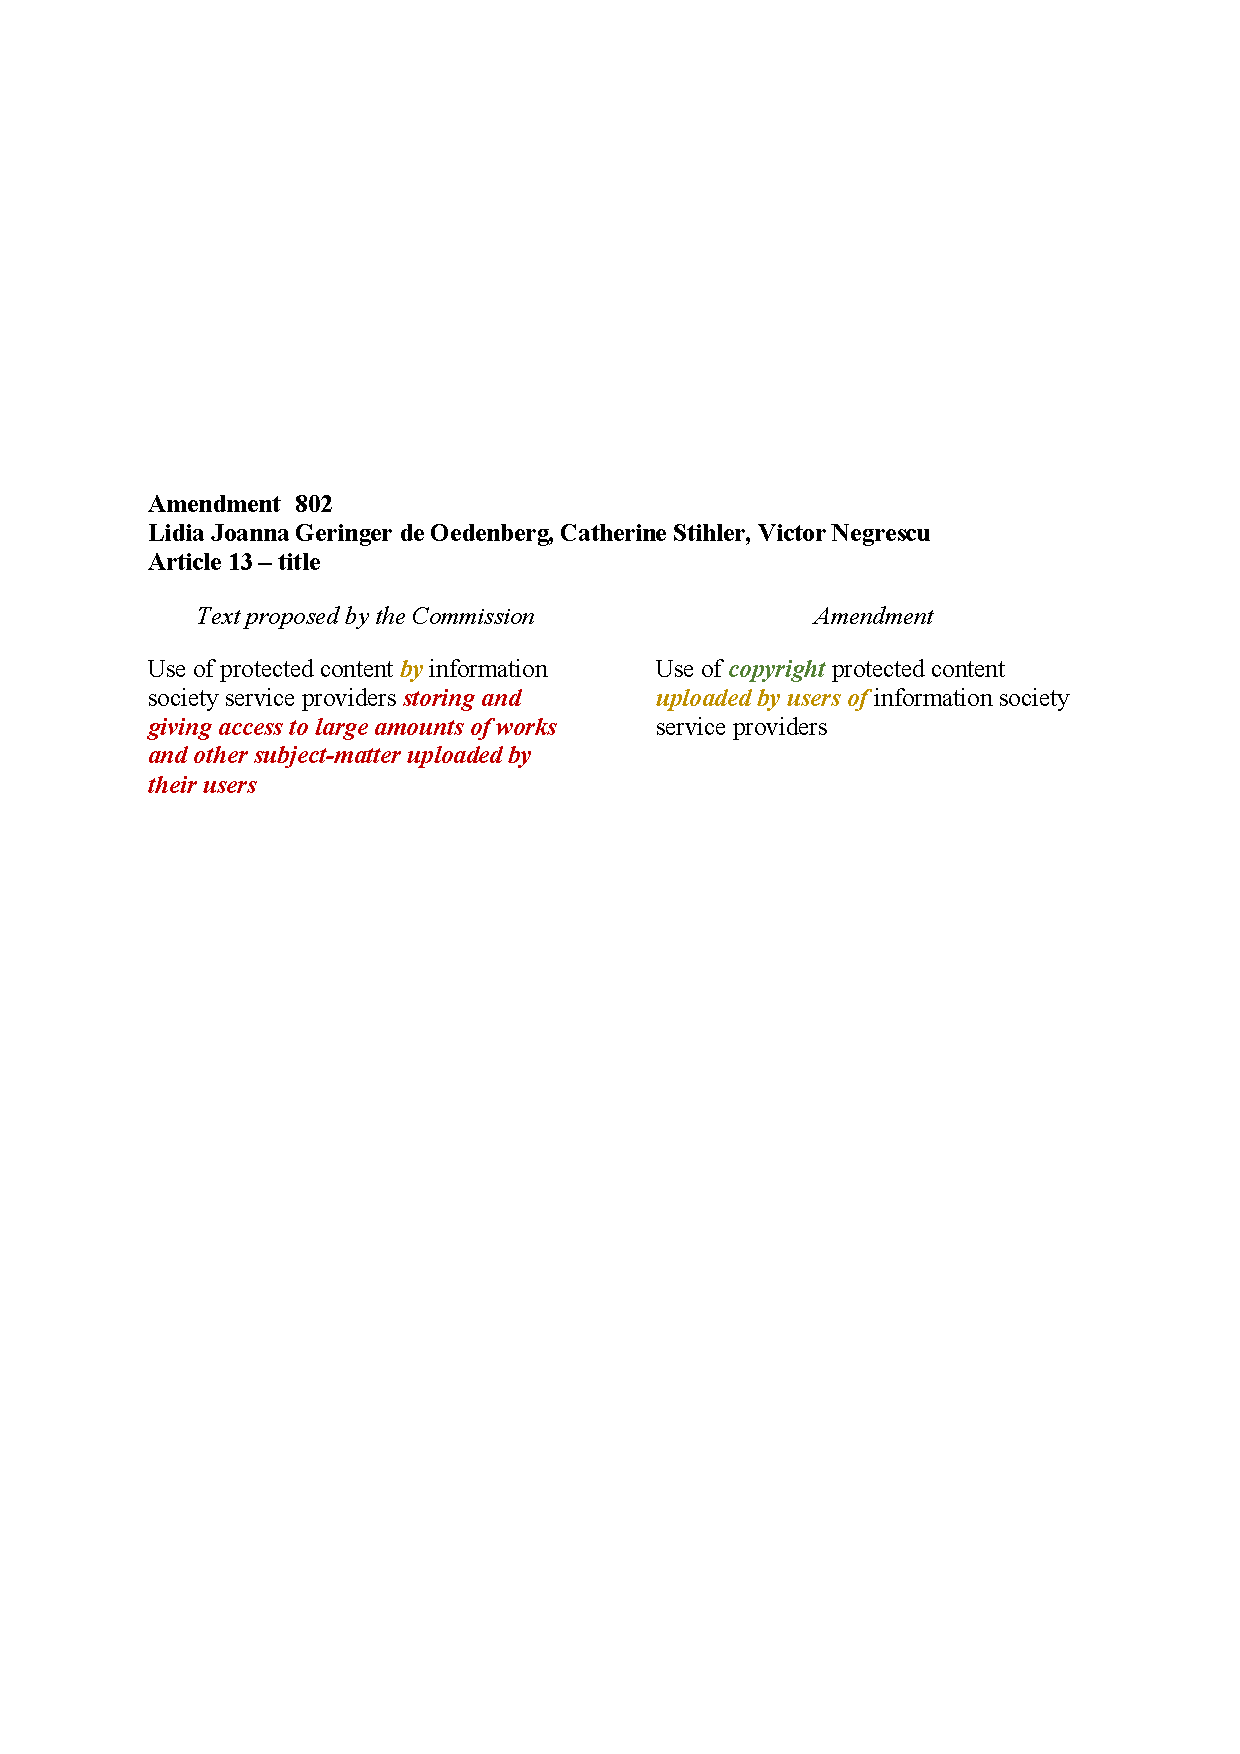
\includegraphics[width=\imgscale]{lmp-amendment-802-colors}}%
	}%
	\vfill
	\vspace{4pt}
	{%
		\setlength{\fboxsep}{5.5pt}%
		\setlength{\fboxrule}{0.5pt}%
		\fbox{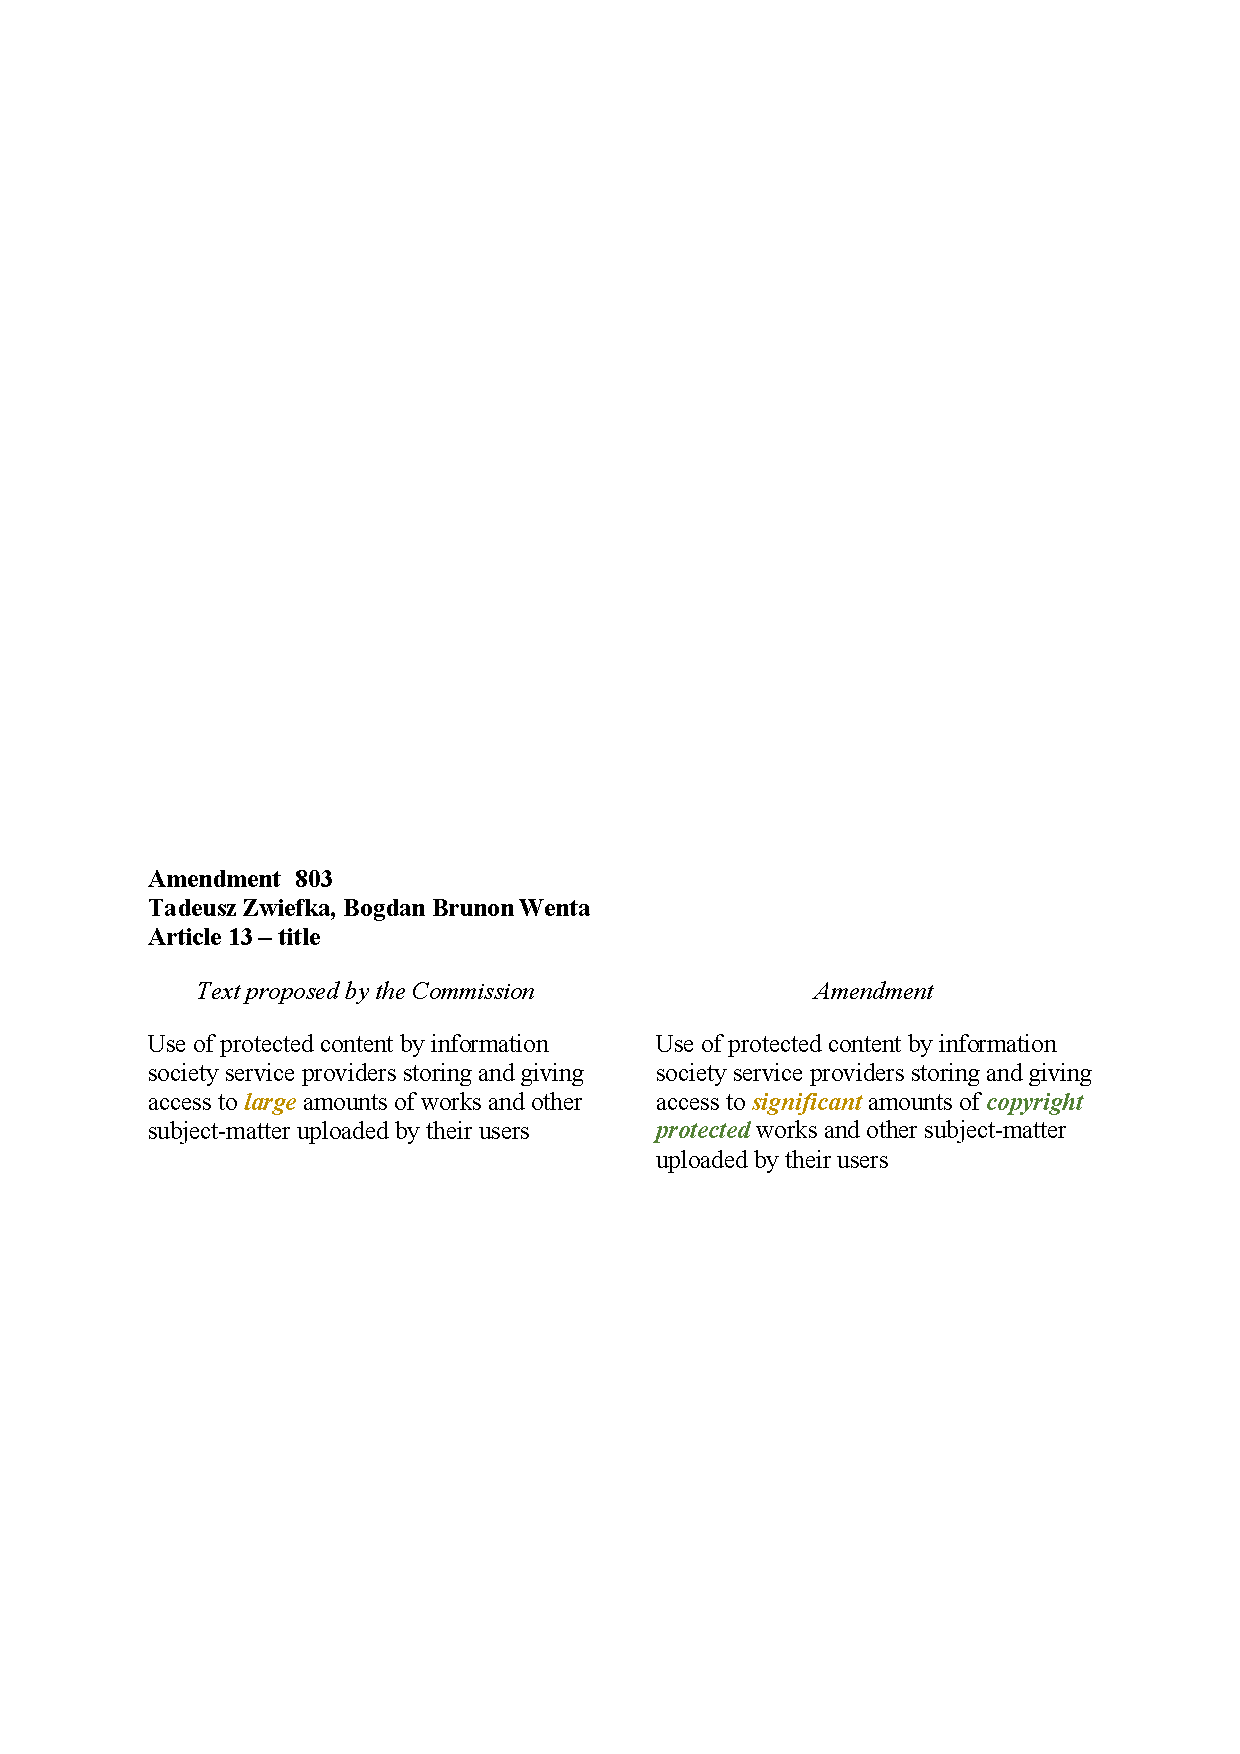
\includegraphics[width=\imgscale]{lmp-amendment-803-colors}}%
	}%
	\caption{
		Example of two conflicting amendments in their raw format on the title of Article 13 of a proposal about copyrights on the Internet.
		(Top) Amendment 802 is proposed by three MEPs and consists of three edits.
		(Bottom) Amendment 803 is proposed by two other MEPs on the same text, and it consists of two edits.
		The last edit of Amendment 802 (deleting the end of the title) conflicts with both edits of Amendment 803.
		Only the first edit of Amendment 803 (replacing ``large'' by ``significant'') was accepted, and all other edits were rejected.
	}
	\label{lmp:fig:amendment}
\end{figure}

\paragraph{Edits}
MEPs propose amendments on a specific article of the legislation, and they can modify several parts within a single amendment.
As a result, we decompose the difference between the original and the amended text into one or several \emph{edits}, as defined below.
An edit is a sequence of words that are inserted or deleted or both.
We extract edits by computing the \emph{diff}, \textit{i.e.}, the difference between the words in two texts, between the original and the amended text of each amendment.
We normalize the texts by removing special characters and by putting the words in lower case.
We keep punctuation because the structure of sentences is important in legal texts.
We merge identical edits proposed by different MEPs, thus considering them as one edit proposed by all authors together.
This is in line with Rule 174 of the Rules of Procedure of the Parliament \cite{europarl2018rule174}.
We extract \numprint{200407} edits for EP7 and \numprint{249086} edits for EP8.
On average, there are 1.85 and 1.93 edits per amendment for EP7 and EP8, respectively.
There are also more dossiers in EP7 than in EP8, which means that there are proportionally more edits per dossier in EP8.

\paragraph{Conflicts}
There exists an inherent competition between the MEPs in the amending process, as amendments are vehicles of political ideas and interests.
We are therefore interested in the conflicts between edits.
We define a \emph{conflict} as a set of edits that overlap.
Edits overlap because they modify parts of the text at the same position.
We extract \numprint{40302} conflicts for EP7 and \numprint{56298} for EP8.
Adding the conflicts to isolated edits, we obtain a dataset of \numprint{126417} data points for EP7 and \numprint{141034} data points for EP8.

\paragraph{Labels}
The votes on each edit are not publicly available, and we need to infer their outcomes from the raw data.
Reports and opinions contain only the amendments accepted within the committees.
Draft reports, draft opinions, and other documents containing all proposed amendments are published separately.
Therefore, if the edits extracted from the latter documents  appear in the former documents, we label them as \emph{accepted}, \textit{i.e.}, the committee votes to include these edits in their report or opinion.
Otherwise, we label them as \emph{rejected}.
Out of the proposed edits, 37.7\% are accepted for EP7 and 25.7\% for EP8.

\paragraph{Timestamps}
The timeline of the legislative process described in Section~\ref{lmp:sec:background} varies from one dossier to another.
Depending on the dossier, MEPs can propose edits during a window of one to six months, after which all the edits related to that dossier are published together.
As a result, the actual, detailed chronology of the edits is unfortunately hidden, and we do not have access to the precise time the edits are proposed and when they are voted.
Furthermore, there is a delay between the time an edit is proposed and the time it is voted: recent edits might be voted \emph{before} older ones.
The timestamps associated with each edit are, therefore, noisy.

%This departs from reality, because we do not have access to the precise time the edits are proposed and when they are voted.
%We only know when a proposal has reached a reporting committee (respectively, an opinion committee), and when the report (respectively, the opinion) is transferred to the Parliament (respectively, the reporting committee).
%In Section~\ref{lmp:sec:cold-start}, we will explore ways of emulating an amending process that is closer to the actual process.
%As shown in Section~\ref{lmp:sec:results}, these simplistic assumptions enable us, nonetheless, to take advantage of the available data to gain insights into the EU legislative process.


In total, we collect \numprint{449493} edits from \numprint{237177} amendments in the European Parliament during the 7\th and the 8\th legislature periods\footnote{We do not collect data from EP9 (2019 -- 2023), as the amount of published data is too small at this time: The legislature period started in Fall 2019 and the Parliament's activities were slowed down due to the COVID-19 crisis in Spring 2020.} (referred to as EP7 and EP8), between 2009 and 2019 (each period lasts 5 years).
After gathering the edits according to the conflicts, we obtain \numprint{267451} conflicts for both EP7 and EP8, covering 1889 dossiers.
We summarize this dataset in Table~\ref{lmp:tab:dataset}.

\begin{table}
  \centering
	\caption{Descriptive statistics of our extended dataset.}
	\label{lmp:tab:dataset}
	\begin{tabular}{lrr}
		\toprule
    & EP7 (2009--2014) &EP8 (2014--2019) \\
		\midrule
  \# amendments & \numprint{108292} &\numprint{128885}  \\
 \# edits       & \numprint{200407} &\numprint{249086}  \\
 \# conflicts   & \numprint{126417} &\numprint{141034}  \\
 \# MEPs        & \numprint{761}    &\numprint{791}     \\
 \# dossiers    & \numprint{1089}   &\numprint{800}     \\
 \% accepted    & 37.7\%            &25.7\%             \\
 \% inserted    & 37.8\%            &37.9\%             \\
 \% deleted     & 22.0\%            &22.4\%             \\
 \% replaced    & 40.2\%            &39.7\%             \\
		\bottomrule
	\end{tabular}
\end{table}

\subsection{Explicit Features}

% - What we add and how we collected these data.
%   - Give an example of an amendment
%   - Explain what are the explicit (meta) features and the text features.
We extract explicit (meta) features of the MEPs, the edits, and the dossiers, as well as text features.
For each MEP, we collect their nationality (one of 28), their EU political group (one of 8 or 9), and their gender.
A political group clusters national parties that share similar political ideologies.
For each edit, we identify whether it is an insertion, a deletion, or a replacement of some words in the proposal, and we compute its length.
We also collect information about where in the law the edit was proposed: in an article (in the body of the proposal), in a recital (in the preamble of the proposal), in an annex, or in other more specific but less frequent parts of a law.
We determine whether an edit in a reporting committee comes from an opinion committee (in which case it is an ``outsider'').
Finally, we note whether an edit comes with an optional justification.
For each dossier, we identify its type (report or opinion) and the committee that is in charge.
We also note if the proposal is a regulation (legally binding for all member states of the EU), a directive (sets general goals that member states can implement however they want), or a decision (binding to one member state or company only).
We describe these explicit features in Table~\ref{lmp:tab:features}.

\begin{table}
  \centering
	\caption{List of features for MEPs and edits.}
	\label{lmp:tab:features}
	\begin{tabular}{lll}
		\toprule
		Category & Feature            & Type [Values]                     \\
		\midrule
		MEP      & Nationality        & Categorical [28]                  \\
		         & Political group    & Categorical [8 or 9]              \\
		         & Gender             & Categorical [2]                   \\
		% & Age                 & Categorical [8 or 9] \\
		% & Experience          & Categorical [8 or 9] \\
		         & Rapporteur         & Binary                            \\
		Edit     & Edit type          & Categorical [3]                   \\
		         & Log-length (+)     & Numerical [$\mathbf{R}_{\geq 0}$] \\
		         & Log-length (-)     & Numerical [$\mathbf{R}_{\geq 0}$] \\
		         & Article type       & Categorical [7]                   \\
		         & Outsider committee & Binary                            \\
		         & Justification      & Binary                            \\
		Dossier  & Type               & Categorical [2]                   \\
		         & Committee          & Categorical [35]                  \\
		         & Legal act          & Categorical [3]                   \\
		%         & Directorate-General & Binary \\
		%         & Subject matter      & Binary \\
		%         & Length of proposal  & Binary \\
		\bottomrule
	\end{tabular}
\end{table}

\subsection{Text Features}

We further augment the dataset by collecting text features of the edit itself.
It is reasonable to expect that certain words and phrases are predictive of the success of an edit.
We extract the deleted words~$w_-$ from the proposal and the inserted words~$w_+$ from  the amendment.
In Figure~\ref{lmp:fig:amendment}, for example, Edit (b) of Amendment 802 has~$w_- = \textit{``by''}$ and~$w_+ = \textit{``uploaded by users of''}$.
We also consider the context of an edit by extracting the original text of the whole amended article.
For Amendment 802, the context is the portion of text labelled as \textit{``Text proposed by the Commission''}.
Finally, we also extract the title of the law proposal; we will use it as a text feature of the dossier.
For Amendments 802 and 803, the title is \textit{``Copyright in the Digital Single Market''}.
We map all words to lower case, and we replace digits in the title by the letter ``D'', as there are many reference numbers that are unlikely to be useful for our task.

We give some statistics of the distribution of the length of the deleted text~$w_-$, the inserted text~$w_+$, the context, and the title in Table~\ref{lmp:tab:text}.
We report the lower quartile~$Q_1$ and the upper quartile~$Q_3$, as well as the median.
About half of the inserted and deleted texts are short (7 words or less), but the distribution of lengths has a long tail, as shown by the larger values of the upper quartile~$Q_3$.
The context provides large portions of text (the median is at 42 for EP7 and 49 for EP8), which will be useful for making predictions.
In Section~\ref{lmp:sec:models}, we describe how we incorporate the explicit features and the text features into our models.

\begin{table}
  \centering
	\caption{Distribution of text lengths in number of words.}
	\label{lmp:tab:text}
	\begin{tabular}{llrrr}
		\toprule
		Legislature & Type            & $Q_1$ & Median & $Q_3$ \\
		\midrule
		EP7         & Insertion $w_+$ & 2     & 7      & 20    \\
		            & Deletion $w_-$  & 2     & 6      & 26    \\
		            & Context         & 15    & 42     & 79    \\
		            & Title           & 6     & 12     & 19    \\
		EP8         & Insertion $w_+$ & 2     & 6      & 17    \\
		            & Deletion $w_-$  & 2     & 6      & 28    \\
		            & Context         & 20    & 49     & 93    \\
		            & Title           & 6     & 10     & 22    \\
		\bottomrule
	\end{tabular}
\end{table}

%- Describe the text (give some descriptive statistics, some plots, ...).
% - Distribution of edit length
% - How many amendments have justification
% - Most frequent words and bigrams
% - Count identical edits/amendments
